%====================================================================================
% LaTeX Document Class and Packages (pLaTeX version)
% 文書クラスとパッケージの読み込み (pLaTeX対応版)
%====================================================================================
\documentclass[10pt]{jsarticle}
\usepackage{cmlab_4.00}				%% 研究室や学会指定のパッケージ
\usepackage{cmlabplus}				%% 拡張パッケージ
\usepackage[dvipdfmx]{graphicx}	    %% 図の貼り付け用パッケージ
\usepackage{url}
\usepackage{balance}
\usepackage{subcaption}
\captionsetup[sub]{labelfont=sf}
\captionsetup{labelsep=quad}
\pagestyle{cmlabw}


\usepackage{amsmath,amssymb}
\usepackage{float}
%\pagestyle{cmlab}
\renewcommand{\figurename}{図 -  }
\renewcommand{\tablename}{表 - }
\renewcommand{\refname}{参考文献}



% 必要に応じて追加のパッケージを読み込みます
% \usepackage{amsmath} % 高度な数式用
\usepackage{tikz} % フローチャート作成用
\usetikzlibrary{shapes,arrows,positioning,calc}

%====================================================================================
% Document Start
% ドキュメント本体の開始
%====================================================================================
\begin{document}

% 2段組設定とタイトル・著者情報
% \twocolumn[...] の中は1段組で表示されます
\twocolumn[%
	\presendate{1}{2025}{8}{8}  %% 発表日 (第1回/2025年/8月/8日)
    \papertitle{幾何音響理論に基づく高速鉄道騒音のリアルタイム可聴化システムの構築}
    \writer{r}{中央大学理工学部都市環境学科 学部4年\quad 増田 樹 \\ Tatsuki Masuda}
]

%**********************************************************
\section{はじめに}
リニア中央新幹線に代表される浮上式高速鉄道は,国家的プロジェクトとして本州を横断する形で建設が進められている.しかし,このような大規模プロジェクトは沿線住民の理解と合意形成なくしては成り立たない.特に,住民が抱える大きな不安の一つに「騒音問題」が挙げられる.

そこで本研究室では,騒音問題を工学的に評価し,効果的な対策の立案や住民への説明に資することを目的として,騒音シミュレーション技術の開発に取り組んできた.既往研究では,据え置き型の大型VRシステム(CAVE)を用いることで,没入感の高い騒音評価環境を構築してきた.しかし,このシステムは体験場所が限定されるという課題があった.

そこで近年,HMD(ヘッドマウントディスプレイ)であるMeta Quest 3を用いた携帯型騒音評価システムの基盤構築が進められてきた.しかし,Meta Quest 3での高音圧騒音シミュレーションにおいて深刻な音割れ問題が発生し,実用化の大きな障壁となっていた.

本研究では,この音割れ問題の根本的解決に取り組み,実用的なシステムの構築を目的とする.これにより,騒音問題に対する合意形成プロセスへの貢献が期待される.

%**********************************************************
\section{浮上式高速鉄道騒音評価システム}
\subsection{システム概要}
本システムは,HMD(ヘッドマウントディスプレイ)としてMeta Quest 3を用いた浮上式高速鉄道騒音評価システムである.従来の据え置き型大型VRシステム(CAVE)とは異なり,Meta Quest 3を使用することで場所を選ばずに手軽に騒音体験が可能な環境を提供する.本研究では,このシステムにおける音割れ問題を解決し,実用的な高品質音響出力を実現した.

\subsection{開発環境}
本研究では,統合開発環境としてUnityを使用し,開発キットとしてXR Interaction Toolkitを使用した.デバイスには,HMDとしてMeta社製のMeta Quest 3を使用した.Unityのバージョンは,開発過程において音響処理の改善のため段階的に移行を実施した.

\subsection{システム構成}
本システムのフローチャートを図\ref{fig:system_flow}に示す.入力データとして車両走行条件,音源の音響パワーレベル,構造物や軌道の形状が設定され,時間ループ内で音源位置と観測者位置がMeta Quest 3の内蔵トラッキング機能から取得され,幾何音響理論に基づき騒音レベルが計算される.

可視化システムでは,UnityとXR Interaction ToolkitでVR空間を構築し,観測者位置で音圧レベルを評価できる.可聴化システムでは,幾何音響理論を基に音圧を計算し,Meta Quest 3の内蔵スピーカーまたはヘッドフォンを通じて立体音響信号として出力される.

VRデバイスには図\ref{fig:meta_quest3}に示すMeta Quest 3を使用する.この装置は,4つのアウトサイドイン・トラッキングカメラ,高解像度ディスプレイ(片目2064×2208),Snapdragon XR2 Gen 2プロセッサ,空間オーディオスピーカーから構成される.Meta Quest 3は完全ワイヤレスでの動作が可能であり,6DoF(6自由度)トラッキングにより高精度な位置・姿勢検出を実現している.

\begin{figure}[h]
\centering
\begin{tikzpicture}[
  node distance=1.2cm,
  box/.style={rectangle, draw, minimum width=2.8cm, minimum height=1.0cm, text centered, font=\scriptsize, align=center},
  input/.style={box, fill=green!20, rounded corners=3pt},
  process/.style={box, fill=blue!20},
  calc/.style={box, fill=yellow!20},
  output/.style={box, fill=orange!20, rounded corners=3pt},
  system/.style={box, fill=gray!20},
  arrow/.style={->, thick, >=stealth}
]

% 入力データ層
\node[input] (input1) {車両走行条件\\設定};
\node[input, right=1.5cm of input1] (input2) {音源の音響\\パワーレベル};
\node[input, right=1.5cm of input2] (input3) {構造物・軌道\\形状データ};

% Time Loop内の処理
\node[process, below=1.8cm of input1] (track1) {音源位置\\トラッキング};
\node[process, right=1.5cm of track1] (track2) {観測者位置\\トラッキング};

% 音響計算部分
\node[calc, below=1.5cm of track1] (calc1) {幾何音響理論\\に基づく計算};
\node[calc, right=1.5cm of calc1] (calc2) {騒音レベル\\計算};

% システム出力
\node[system, below=1.5cm of calc1] (vis) {可視化\\システム};
\node[system, right=1.5cm of vis] (audio) {可聴化\\システム};

% 最終出力
\node[output, below=1.5cm of vis] (screen) {スクリーン\\表示};
\node[output, right=1.5cm of screen] (vr) {VR空間\\構築};
\node[output, right=1.5cm of vr] (speaker) {スピーカー\\音響出力};

% Time Loopの枠
\draw[dashed, thick, blue] ($(track1.north west) + (-0.5,0.5)$) rectangle ($(calc2.south east) + (0.5,-0.5)$);
\node[above right=0.1cm and -1.5cm of track1.north west, font=\small\bfseries, color=blue] {Time Loop};

% 矢印の描画
\draw[arrow] (input1) -- (track1);
\draw[arrow] (input2) -- (calc1);
\draw[arrow] (input3) -- (calc1);
\draw[arrow] (track1) -- (calc1);
\draw[arrow] (track2) -- (calc2);
\draw[arrow] (calc1) -- (calc2);
\draw[arrow] (calc2) -- (vis);
\draw[arrow] (calc2) -- (audio);
\draw[arrow] (vis) -- (screen);
\draw[arrow] (vis) -- (vr);
\draw[arrow] (audio) -- (speaker);

% 横の矢印
\draw[arrow] (track1) -- (track2);
\draw[arrow] (calc1) -- (calc2);
\draw[arrow] (vis) -- (audio);
\draw[arrow] (screen) -- (vr);
\draw[arrow] (vr) -- (speaker);

\end{tikzpicture}
\caption{浮上式高速鉄道騒音評価システムの構成}
\label{fig:system_flow}
\end{figure}

\subsection{幾何音響理論に基づく音響計算}
本研究では,日本音響学会道路交通騒音調査研究委員会のASJ RTN-Model 2018を用いて音響計算を行う.これは幾何音響理論に基づき,音源を半自由空間の点音源として扱うモデルである.

\subsubsection{基本計算式}
ASJモデルにおいて,受音点での音圧レベル$L_p$(dB)から音源の音響パワーレベル$L_W$(dB)を算出する式は以下の通りである:
\begin{equation}
L_W = L_p + 20\log_{10}r + 8 - \Delta L_{cor}
\end{equation}
ここで$r$は音源から受音点の距離,$\Delta L_{cor}$(dB)は回折や指向性による減衰の補正量である.

\subsubsection{音圧レベルの合成}
受音点での音源からの伝播音の圧力レベルの合成値$L_p$(dB)は次式で表される:
\begin{equation}
L_p = 10\log_{10}\sum_{i=1}^{n}(10^{L_{pi}/10})
\end{equation}
ここで$i$は合成する音源の数である.

\subsubsection{物理現象の考慮}
本システムでは以下の物理現象を考慮した音響計算を実装している:
\begin{itemize}
\item 距離減衰:$20\log_{10}(r)$による減衰
\item 大気吸収:空気中での音波エネルギー損失
\item 回折効果:遮音壁による音の回り込み(Maekawaチャートに基づく計算)
\item ドップラー効果:$f' = f \cdot \frac{c}{c - v_s \cos\theta}$による周波数変化
\end{itemize}

\subsubsection{構造物音の考慮}
走行時の車外騒音には,空気圧変動による空力音と,構造物振動による構造物音が影響を与える.本システムでは,より現実的な騒音環境を再現するため,構造物音を明示的に考慮したシミュレーションを実装している.

構造物音は,走行中に発生する空力音に連動して移動する無指向性の仮想点音源として取り扱う.各走行音源位置から一定距離下方(本研究では1.5m下)に無指向性の仮想点音源を配置し,構造物振動による音響寄与を再現する.

構造物音の音響パワーレベル$L_{W,str}$は走行速度の関数として次式で表される:
\begin{equation}
L_{W,str} = a + 30 \log_{10} V
\end{equation}
ここで,$V$は走行速度(km/h)で,定数$a$は橋種ごとに決定される.本研究では,コンクリート橋の箱桁構造を想定し定数$a$は35.9を用いた.走行速度500km/hの場合,仮想点音源の音響パワーレベルは114.8dBとなる.

この構造物音の考慮により,単純な空力音のみのシミュレーションと比較して,より実際の高速鉄道走行時に近い複合的な音響環境を構築することが可能となった.

%**********************************************************
\section{Meta Quest 3における音響処理問題と解決手法}
\subsection{音割れ問題の発見と原因分析}
本研究において最初に直面した最大の技術的課題は,Meta Quest 3でのリニアモーターカー走行音シミュレーションにおいて深刻な音割れが発生することであった.この問題は,システムの実用性を著しく損なう重大な障害となっていた.

詳細な検証の結果,以下の条件において音割れが顕著に発生することが判明した:
\begin{itemize}
\item リニアモーターカーから受音点までの距離が近距離(5m以内)の場合
\item 車両編成数が多い場合(特に16両編成時)
\item 複数音源が同時に高音圧レベルで再生される状況
\end{itemize}

詳細な解析により,音割れの根本原因がUnityのAudio Mixerにおける音圧レベル範囲制限(-80dB〜0dB)にあることを特定した.この制約により,高音圧データ処理時にクリッピングが発生し,音質劣化を引き起こしていた.

\subsection{体系的解決手法の検討と効果検証}
音割れの根本原因を解明するため,原因仮説を体系的に分類し,各仮説に対する検証手法を実施した.\textbf{図-\ref{fig:audio_distortion_solutions}}に音割れ問題の原因仮説分類と検証結果を示す.

%\begin{figure}[t]
	%\begin{center}
		%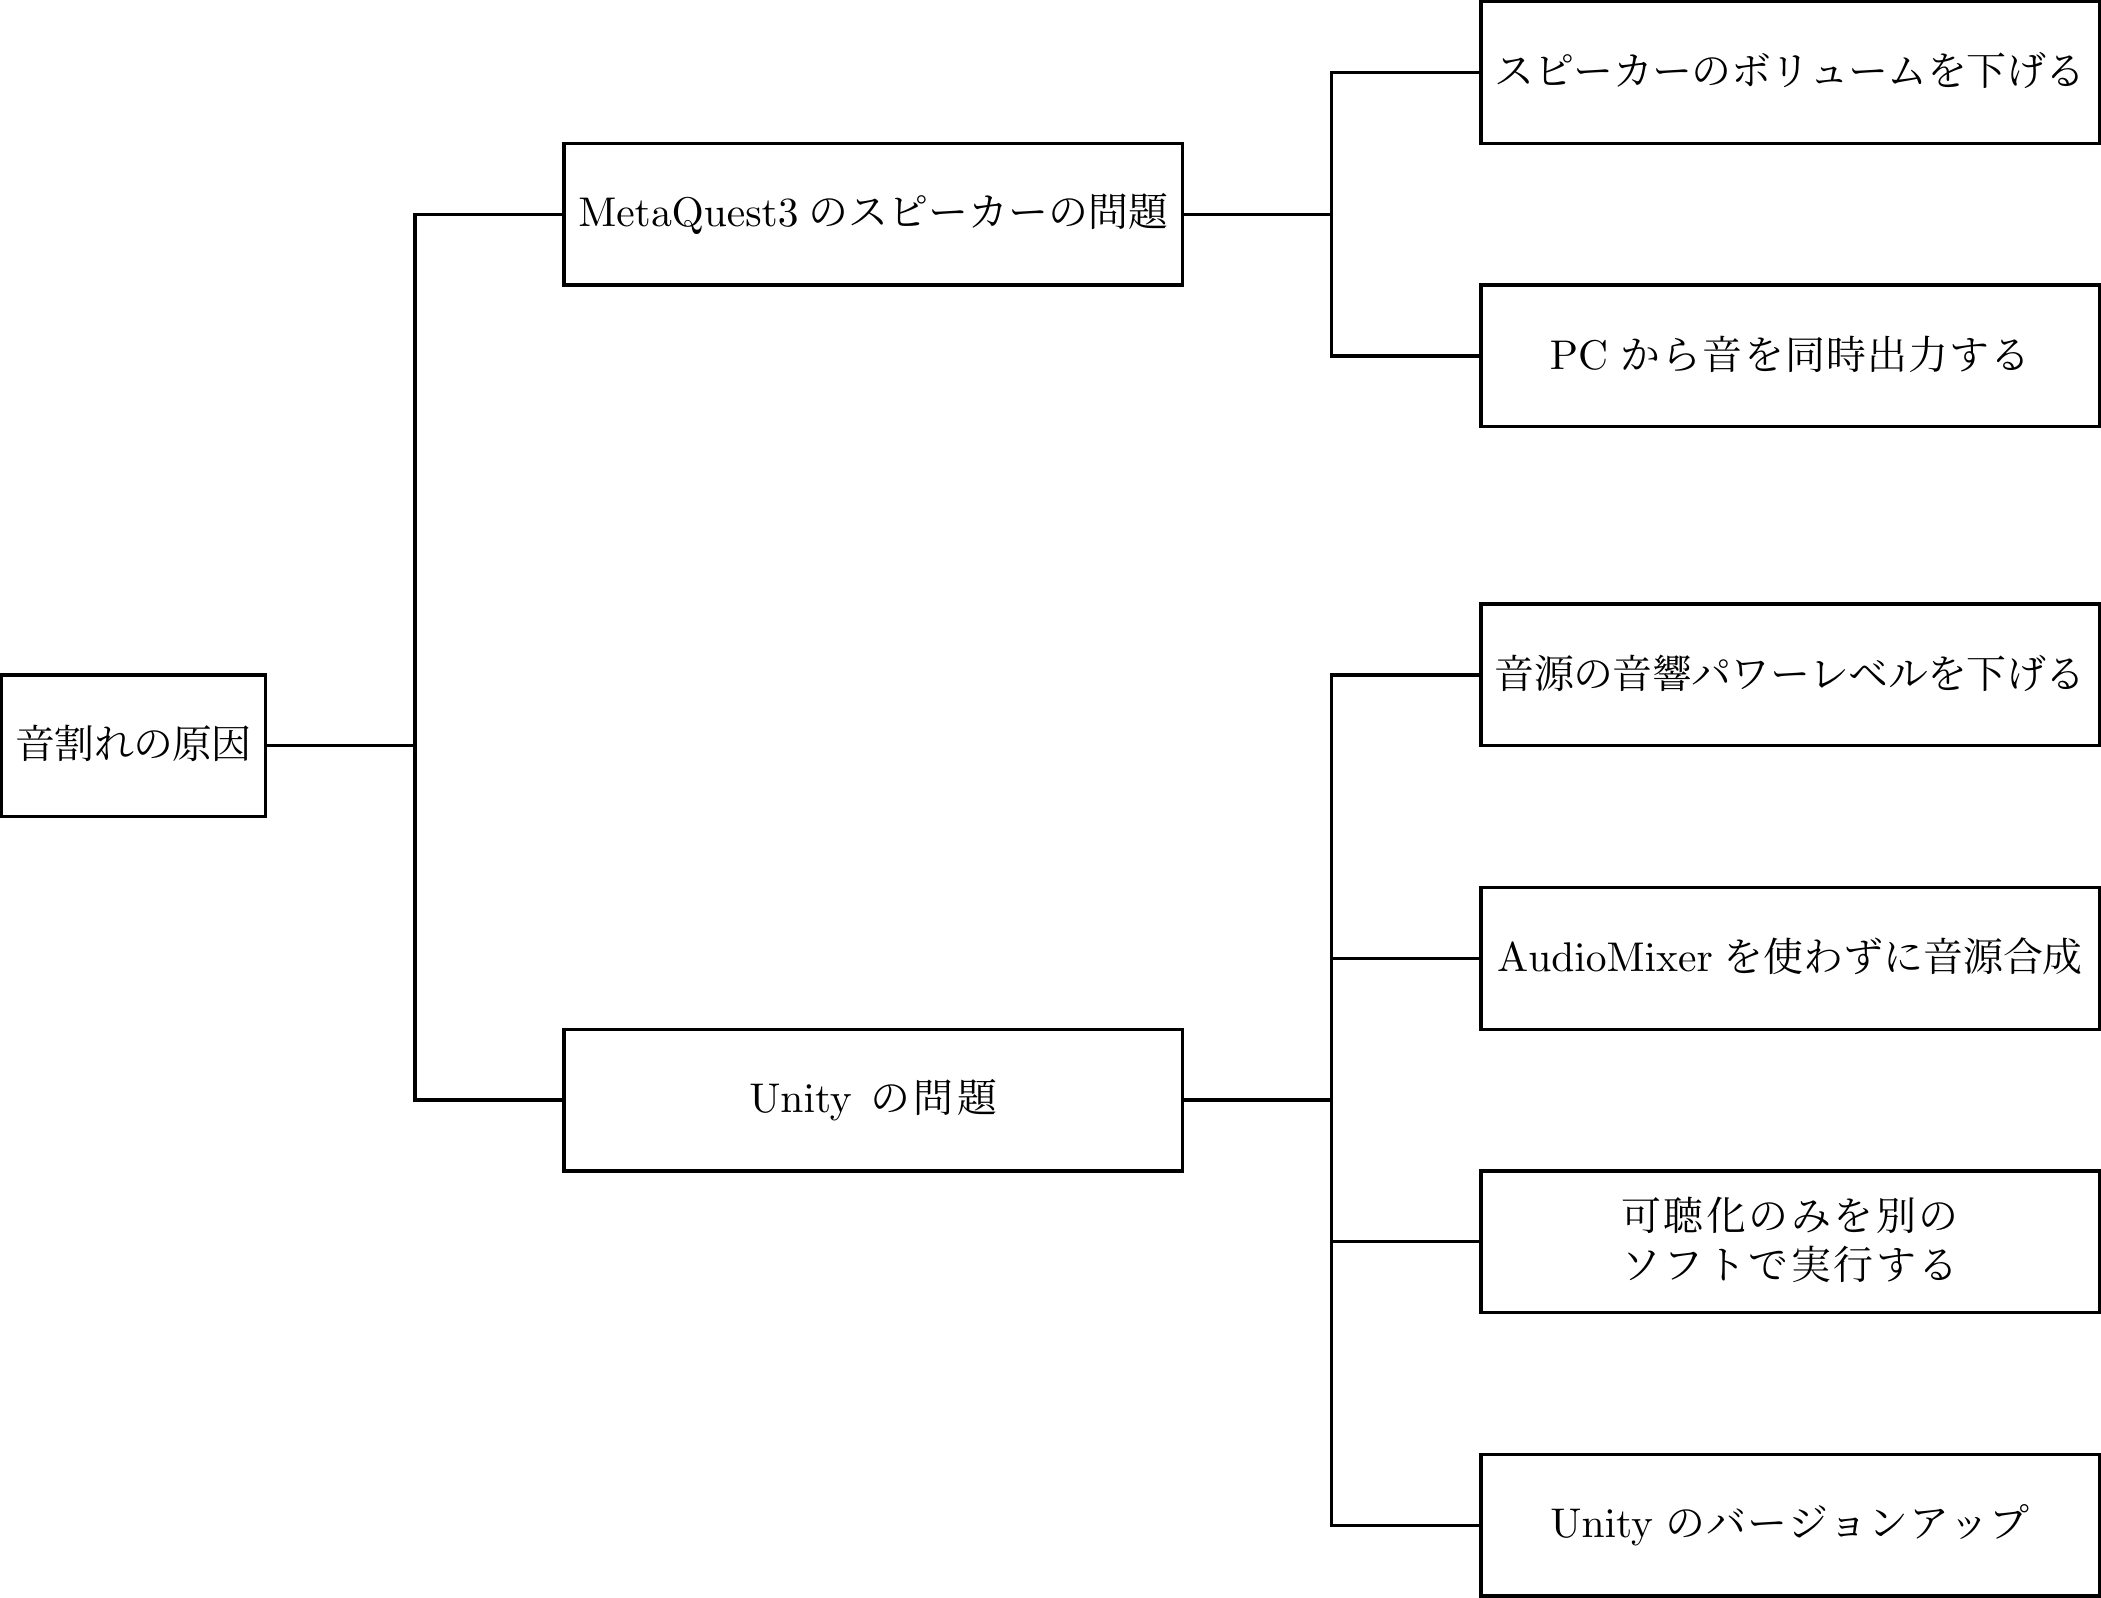
\includegraphics[width=0.5\linewidth]{pic/audio_distortion_flowchart.png}
		%\caption{音割れ問題の原因仮説分類と検証手法}
		%\label{fig:audio_distortion_solutions}
	%\end{center}
%\end{figure}

\begin{figure}[t]
\begin{center}
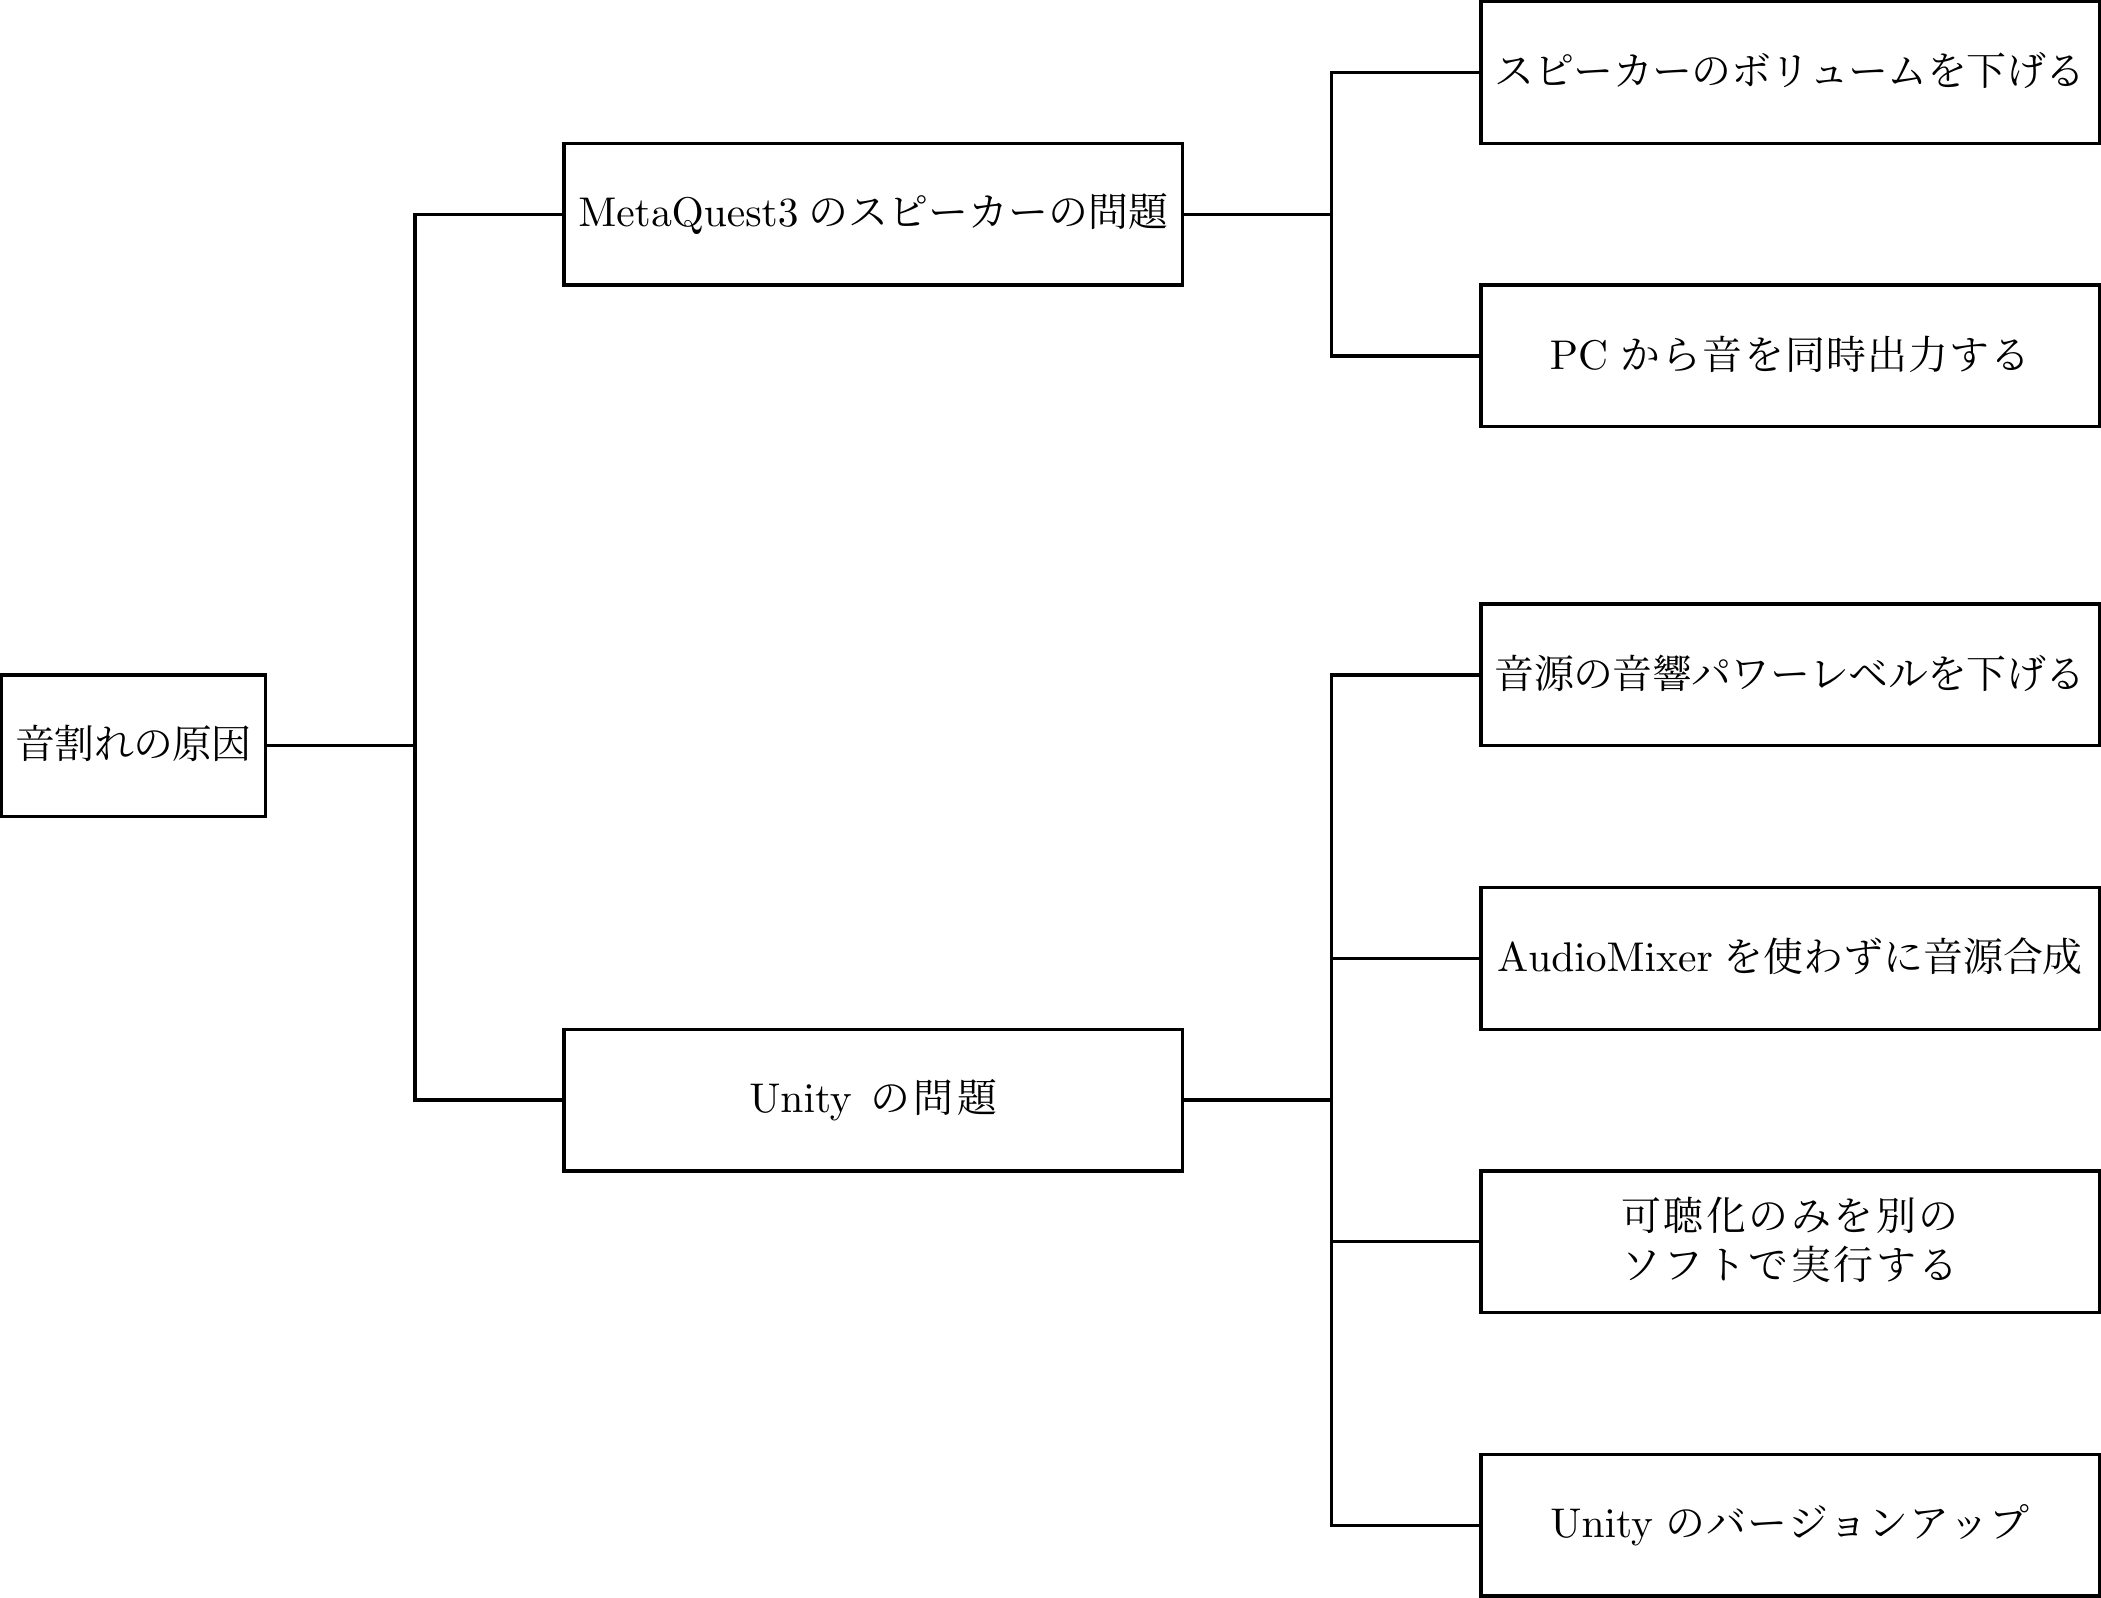
\includegraphics[width=0.9\linewidth]{pic/audio_distortion_flowchart.png}
%\vspace{-0.3cm}
\caption{音割れ問題の原因仮説分類と検証手法}
\label{fig:audio_distortion_solutions}
\end{center}
\end{figure}

音割れ問題の原因仮説を「ハードウェア問題」と「ソフトウェア問題」の2つに大分類し,各仮説に対して以下の6つの検証手法を実施した:

\textbf{ハードウェア問題仮説の検証}

\textbf{手法1:Meta Quest 3本体音量調整}
デバイス本体の音量設定を段階的に低下させたが,音割れの改善は認められなかった(効果:×).

\textbf{手法3:Meta Quest Link PC出力}
PC接続を通じた外部音響出力を検討したが,最終的な音響処理がUnityのAudio Mixerを経由するため,根本的な解決には至らなかった(効果:×).

\textbf{ソフトウェア問題仮説の検証}

\textbf{手法2:車両音源音圧レベル調整}
音源の音響パワーレベルを120dBから110dBへ変更により音割れは部分的に軽減されたが,全体的な音圧が不十分となり,リアリティの観点から実用的ではなかった(効果:△).

\textbf{手法4:Audio Mixer回避独自プログラム開発}
Audio Mixerを使用しない独自の音源合成アルゴリズムを開発.音圧レベル(dB)から線形スケール(0〜1)への変換処理により,各音源データのvolumeパラメータへ直接適用する手法で,16両編成車両による近距離シミュレーションにおいて音割れの大幅な改善を確認した(効果:○暫定的解決).

\textbf{手法5:OSC通信外部デバイス連携}
UDP通信による外部音響デバイスとの連携を検討段階として位置づけた(効果:?検討段階).

\textbf{手法6:Unity移行}
Unityエンジンのバージョン移行により音割れ問題が根本的に解決された(効果:◎根本的解決).

この検証結果から,音割れ問題の原因は「ソフトウェア問題」であり,特にUnity 2023年版で実装されたAAudioドライバによる根本的改善が決定的な解決策であることが判明した.

\subsection{Unity移行による根本的解決}
多様な対処法を検討した結果,最終的にUnityエンジンのバージョン移行により音割れ問題が根本的に解決された.Unity 2021.2.19f1からUnity 6000への段階的移行を実施し,特にUnity 2023年版で実装されたAAudioドライバが決定的な改善をもたらした.

従来のOpenSL ESアーキテクチャと比較して,AAudioドライバは以下の技術的優位性を提供した:
\begin{itemize}
\item \textbf{バッファオーバーフロー防止}:高音圧データ処理時の安定性向上
\item \textbf{ハードウェア直接制御}:中間層を排除した効率的データ転送
\item \textbf{低レイテンシ処理}:リアルタイム音響シミュレーションに最適化
\item \textbf{マルチソース対応}:複数音源の同時高品質再生
\end{itemize}

Unity 6000への移行完了後,従来問題となっていた全ての条件(16両編成・近距離5m・高音圧レベル)において音割れが完全に解消された.これにより,Audio Mixer回避やOSC通信等の複雑な回避策が全て不要となり,シンプルで安定したシステム構成を実現した.

%**********************************************************
\section{おわりに}
本研究では,Meta Quest 3を用いた浮上式高速鉄道騒音評価システムにおける深刻な音割れ問題の根本的解決に取り組み,実用的な高品質VR騒音体験システムの構築を実現した.

解析結果として,音割れ問題の根本原因がUnityのAudio Mixer制約にあることを特定し,5つの対策手法を体系的に検証した結果,Unity 2021から6000への段階的バージョン移行により問題が完全に解決された.主な要因は2023年版で導入されたAAudioドライバによるオーディオ処理の根本的改善と考えられる.

また,本研究により以下の成果が得られた:
\begin{itemize}
\item Unity 2023年版AAudioドライバにより16両編成・近距離(5m)での安定した高音圧シミュレーションが実現された
\item 複雑な回避策(Audio Mixer回避,OSC通信等)が不要となり,シンプルで堅牢なシステム構成を確立した
\item 幾何音響理論に基づく統合的音響計算エンジン(距離減衰,大気吸収,回折効果,ドップラー効果,構造物音)の実装が完了した
\item JR東海との産学連携による6回の技術報告会を通じてシステムの実用性が検証された
\end{itemize}

本システムは,リニア中央新幹線等の大規模インフラプロジェクトにおける騒音影響の事前評価と住民合意形成において重要な役割を果たすことが期待される.

今後は,Mixed Reality技術の導入による現実環境との重畳表示,多様な車両編成・運行シナリオへの対応拡張,さらなる音響計算精度の向上等により,実用性の更なる向上を図る予定である.

%**********************************************************
参考文献
\begin{thebibliography}{9}
\bibitem{ref1} 西航平, 宮内暖季, 樫山和男:VR 技術を用いた浮上式高速鉄道騒音評価システムの高精度化,第 51 回土木学会関東支部技術研究発表会講演概要集,VII-15, 2024.
\bibitem{ref2} 日本音響学会道路交通騒音調査研究委員会:道路交通騒音の予測モデル"ASJ RTN-Model 2023",日本音響学会誌,2023.
\end{thebibliography}

\end{document}
